\documentclass[12pt]{article}

% set indentation
\usepackage{parskip}
%\setlength{\parindent}{16mm}

% for the figures
\usepackage{graphicx}
\usepackage{extsizes}
\usepackage{wrapfig}
\usepackage{leftidx}
\usepackage{amsmath}
\usepackage{dsfont}
% change margins
\usepackage{geometry}
\geometry{left=20mm,right=20mm,top=15mm,bottom=15mm}

% for the reference
\usepackage[sort]{natbib}
\usepackage{url}
\usepackage{placeins}
%\usepackage{authblk}
\usepackage{setspace}
\usepackage{tabularx}
%\doublespacing
% in preamble
%\usepackage{movie15}
% in documenet

\usepackage{authblk}
\usepackage{graphicx}
% My packages
\usepackage{parskip}
\usepackage{relsize, threeparttable}
\usepackage{array}
\usepackage{booktabs}
\usepackage{lscape}
\usepackage{tabularx}
\usepackage{makecell}
\usepackage{booktabs}
\usepackage{numprint}
\usepackage{amsmath}
\usepackage{mathtools}
\usepackage{amssymb}
\usepackage{multirow}
\setlength{\parindent}{16mm}
% for the figures
\usepackage{graphicx}
\usepackage{placeins}
% for the reference
\usepackage{natbib}
\usepackage{floatrow}
\usepackage{chngcntr}
\usepackage{url}
\usepackage{dutchcal}
%\usepackage{boondox-calo}
\usepackage{upgreek}
%\date{}
\usepackage{color,soul}


\setlength{\parindent}{0pt}
\definecolor{lightgrey}{rgb}{0.925, 0.925, 0.925}
\sethlcolor{lightgrey}

\newcommand{\note}[1]{\textcolor{blue}{[#1]}}




\title{Unraveling the time dynamics of life annuities}

\author[1]{Jes\'us-Adri\'an \'Alvarez\thanks{jesusalvarezmtz@gmail.com}}

\author[2]{Andr\'es M. Villegas}

\affil[1]{{\small Independent Researcher} }

\affil[2]{\small{School of Risk and Actuarial Studies\\ UNSW Business School, UNSW Sydney, Australia}}
%\date{}

\begin{document}
\maketitle

{
\setcounter{tocdepth}{2}
%\tableofcontents
}



\begin{abstract}
	
Mortality and interest rates evolve jointly, dynamically influencing the values of life annuities and actuarial reserves. Building on established results from actuarial science and demography, this paper introduces a set of differential equations that simultaneously quantify (i) changes in mortality and interest rates, and (ii) the sensitivity of annuity and reserve values to these changes, measured through entropies and durations.

We illustrate the practical application of our framework by examining the long-term development of life annuity values using data for the United Kingdom from 1841 to 2021. The analysis reveals how financial and longevity risks have evolved over time, uncovering detailed patterns across interest rate terms, age groups, and causes of death. It also highlights a clear interplay between the financial and longevity risk -- where the latter is at times masked by periods of elevated financial volatility.

Our equations explicitly capture the joint dynamics of mortality and interest rates, to better understand the changing economic-demographic environment and its impact on life annuity values. The main contribution of this paper is to provide actuaries with practical, data-driven tools to evaluate and manage evolving risks in life annuity portfolios and actuarial reserves.




	
\end{abstract}

\textbf{Keywords:} entropy, duration, longevity risk, interest rates, Thiele differential equation


\newpage
\section{Introduction}\label{sec:1_introduction}


Pension funds and insurance companies face growing concerns about how simultaneous fluctuations in interest rates and mortality affect the valuation and risk profile of their life annuity portfolios. Two key sources of variation underlie the time dynamics of life annuities. First, there is uncertainty surrounding the future evolution of both mortality and interest rates. Second, there is variation in how life annuities \textemdash and their associated actuarial reserves and capital requirements\textemdash respond to changes in these factors.

The first source of variation has been studied extensively, with a wide range of models proposed to forecast mortality and interest rates from diverse perspectives. However, the second source of variation (i.e., sensitivity of life annuities to fluctuations in mortality and interest rates) has been less explored. While much of the research on interest rate sensitivity has focused on immunisation theory, studies on mortality sensitivity remain limited.

An important contribution in this area comes from \citet{rabitti2020mortality}, who examined how mortality sensitivity varies with interest rates using historical life tables and assuming constant interest rates. Their findings suggest that mortality sensitivity is higher when interest rates are low, with the financial component becoming a key risk when both factors are considered. 
 
Along the same lines, \citet{di2025decomposing} extends the \citet{Vaupel2003} method by employing commutation functions to derive a closed-form expression that links changes in annuity values to changes in mortality rates. The approach assumes a fixed interest rate to compute a financially adjusted entropy to quantify the contribution of changing mortality rates. While this assumption confines the analysis to a constant discounting framework, and potentially affecting the separation of mortality and financial contributions to observed annuity changes, the contribution of \citet{di2025decomposing} remains a significant step forward in integrating mortality dynamics into annuity valuation in the actuarial literature.
 
The analyses by \citet{rabitti2020mortality} and \citet{di2025decomposing} offer important insights into the sensitivities of life annuities to mortality and interest rate changes. However, differences in age-specific mortality improvements and variations along the yield curve may lead to contrasting effects that are not captured in their analyses. Moreover, the dynamics of sensitivity changes over time and their underlying drivers—such as cause-of-death patterns—remain unclear. It is also uncertain whether the sensitivity results in \citet{rabitti2020mortality} and \citet{di2025decomposing} hold when using actual term structures of interest rates.
 

In this article, we build on established actuarial and demographic results to introduce a set of differential equations to address the gap in better understanding the time dynamics of life annuities and their associated reserves. Our approach quantifies the simultaneous contributions of changes in mortality and interest rates, and the sensitivity of life annuities and reserves to these dynamics.

We begin by developing differential equations for a deterministic life annuity factor. These equations are then expanded to disentangle the sources of change into age-group and term-specific attributions, and to identify the causes of death driving these changes. To illustrate the application of our framework, we use United Kingdom data from 1841 to 2021 to analyse the drivers behind long-term changes in life annuity factors. Finally, we generalise our differential equations to the stochastic representation of life annuity reserves, establishing the link with the well-known Thiele differential equation and discussing its applications in risk management.

Our equations are simple, intuitive, and easily applicable, enabling actuaries and risk managers to assess the financial and longevity risks embedded in their life annuity portfolios. From an actuarial perspective, these differential equations provide valuable insights for developing strategies to improve risk management by leveraging well-established concepts from mathematical demography and immunisation theory.

The remainder of the article is structured as follows. In Section \ref{sec:SensitivityMortalityInterest}, we review key results from the actuarial and demographic literature on mortality and interest rate sensitivities. Section \ref{sec:TimeDynamics} presents a set of differential equations for the time dynamics of life annuities in the deterministic case. Section \ref{sec:UK_Illustration} illustrates the application of our equations using historical data from the United Kingdom.  In Section \ref{sec:Reserves}, the equations are extended to the stochastic representation of annuity reserves. Lastly, we conclude with a discussion on the potential applications of the equations developed in this paper. The code to replicate the results and all derivations presented in this article are available in the open-source repository: \textit{link available upon publication}.



\section{Sensitivity to Interest and Mortality Changes}\label{sec:SensitivityMortalityInterest}

\subsection{Duration}

Duration (denoted as $D$) is a foundational metric for assessing the sensitivity of financial instruments to changes in interest rates. Specifically, it quantifies the price sensitivity of a life annuity (or other financial assets such as bonds and fixed-income products) to variations in the force of interest, $\delta$ \citep{milevsky2013life,charupat2016sluggish}. The interpretation of duration varies depending on its context. For instance, Macaulay duration estimates the weighted average time required for an investor to recover a bond's price through its cash flows, while modified duration measures the percentage price change of a bond for a 1\% change in interest rates.

From a mathematical perspective, duration corresponds to the first-order derivative of a financial quantity with respect to $\delta$. The second-order derivative, known as convexity, captures the curvature of the relationship between price and interest rate changes. Both duration and convexity are essential to interest rate immunisation strategies \citep{redington1951papers,fisher1971coping,shiu1990redington,santomero1997financial,courtois2007immunization}, ensuring that portfolios are adequately protected against fluctuations in interest rates.

\subsection{Entropy}\label{sec:Entropy}

In demography, entropy (denoted as $H$) is defined as a measure of the sensitivity of life expectancy to changes in mortality rates \citep{leser1955variations,keyfitz1977difference,demetrius1974demographic,goldman1986new, aburto2019threshold}. Mathematically, the entropy is the first-order derivative of life expectancy with respect to the force of mortality $\mu$. Higher entropy values indicate greater responsiveness of life expectancy to proportional changes in mortality rates.

\citet{Vaupel2003} made a significant contribution by expressing the time derivative of life expectancy at birth, $e(0, t)$, as a function of the pace of reducing mortality, $\rho(t)$, and entropy, $H(t)$:

\begin{equation}\label{eq:lifeexpdecomp}
	\dfrac{\partial e(0,t)}{\partial t} = \rho(t) H(t) e(0,t).
\end{equation}

This formulation underscores the interplay between mortality improvements and the sensitivity of life expectancy. Furthermore, it enables the decomposition of changes in life expectancy into age-specific and cause-specific contributions to both mortality improvement and entropy.

\citet{Haberman2011} extended the concept of entropy to life annuities, defining it as a measure of the sensitivity of a life annuity to proportional changes in the force of mortality. This extension links entropy directly to longevity risk in life annuity portfolios \citep{rabitti2020mortality} and has been applied to analyse socio-economic disparities in pension systems \citep{alvarez2021linking}.

Entropy has also found applications in mortality-immunisation research, where strategies analogous to interest rate immunisation are employed to mitigate the impact of mortality rate changes on portfolio values. Discrete formulas for life annuity entropies and convexities have been derived under the assumption of constant or proportional changes in the force of mortality, $\mu$ \citep{wang2010optimal,tsai2011actuarial,Tsai2013a,Li2011}. These methods have been generalised to a wide range of life insurance and annuity products \citep{li2012key,Li2012,Wong2015,Luciano2015,levantesi2018natural}.

\subsection{Merging Perspectives}

While mortality sensitivity (primarily studied by demographers) and interest rate sensitivity (predominantly examined by actuaries and financial analysts) both aim to understand the drivers of change in life-contingent quantities, these research areas have largely evolved independently. Notable exceptions include studies by \citet{Haberman2011}, \citet{rabitti2020mortality}, \citet{Lin2020}, \citet{alvarez2021linking} and \citet{di2025decomposing}, which bridge these domains. In particular, \citet{Lin2020} advanced this integration by deriving discrete formulas for life annuities and whole life insurance products that account for their sensitivity to simultaneous changes in mortality and interest rates. They introduced a composite variable, termed the ``force of mortality-interest'', defined as $\mu^* = \mu + \delta$. While this approach offers a novel perspective, it assumes that mortality and interest rates change at the same pace, a condition that may not reflect real-world dynamics. 


An important contribution in this direction is made by \citet{di2025decomposing}, who extends the decomposition method of \citet{Vaupel2003} by using commutation functions to derive a closed-form expression for changes in annuity values. %Their decomposition method for the rate of mortality improvement, the numerator of life table entropy, and the covariance between mortality improvement and the annuity factor.
However, their decomposition method assumes a fixed interest rate, which constrains the mortality contributions under a constant discounting framework. Despite this limitation, \citet{di2025decomposing} represents a key advancement in linking mortality dynamics with annuity valuation in the actuarial literature.

In this article, we build on actuarial and demographic literature to develop a set of differential equations that capture the time dynamics of life annuities and reserves through durations and entropies. These equations improve our understanding of how changing economic and demographic conditions affect annuity values and reserves. The core contribution is to equip actuaries with practical tools for evaluating and managing the evolving risks in annuity portfolios and reserves based on real-world data. In the following section, we derive these equations and explore practical applications. 


\section{Time Dynamics of Life Annuities}\label{sec:TimeDynamics}
\subsection{Preliminaries}\label{preliminaries}

In this section, we introduce the time variables and notation required to describe the dynamics of life annuities. Let $(x)$ denote an insured individual aged $x$, where $x \geq 0$. The random variable \( S_x \) represents the future lifetime of $(x)$, such that \( x + S_x \) corresponds to the total lifetime of the individual. 

The actuarial value of the policy associated with life $(x)$ is determined based on information about the economic-demographic environment in which the life annuity is issued. Let \(t\) denote the  time at which this information about the \textit{economic-demographic environment} becomes available. We assume that \(t\) is continuous, reflecting the continuous evolution of this information. Separately, we use  the time variable \(u\) to denote the \textit{time of valuation of the policy}.

Although \( t \) and \( u \) are both time variables, they are not necessarily the same. The economic-demographic information used to evaluate life annuities is indexed by \( t \). However, there may be a lag between the time at which actuarial assumptions are set (denoted by \( t \)) and the time corresponding to the valuation of the policy (denoted by \( u \)). This lag is common, particularly for mortality data, which is often collected by national statistical offices with a delay of several years. In some cases, \( t = u \), such as when companies have access to up-to-date experience data for insured lives or when market interest rates are continuously available. However, this is not always the case.

To explicitly account for this distinction, we differentiate between the two time variables, \( t \) and \( u \), to better analyse the sources of change in life annuities. This distinction is also critical for deriving the differential equations that describe the time dynamics of life annuities and reserves, and is further examined in Section \ref{sec:ThieleEquations}, where we highlight the connection with the Thiele differential equation. In what follows, however, we focus on changes in life annuity values over the time variable \(t\).

\subsection{Changes over Time $t$}

% Let \( I_{s,t} = \mathds{1}_{\{S_x > s,t\}} \) represent the indicator of survival for a life at age \( x \) to time \( s \), with information generated at time \( t \). The expected value \( \mathbb{E}[I_{s,t}] = {}_s p_x(t) \) is the time \( t \) survival probability, i.e., the probability that a person aged \( x \) survives from age \( x \) to age \( x+s \). This probability is given by the expression ${}_sp_x(t)=e^{-\int_{0}^{s}\mu(x+y,t)dy}$, where \(\mu(x,t)\) is the force of mortality at age \(x\) in time $t$.

Let \({}_s p_x(t) \) be the probability that a person aged \( x \) survives from age \( x \) to age \( x+s \), estimated with information at time $t$. This probability is given by the expression ${}_sp_x(t)=e^{-\int_{0}^{s}\mu(x+y,t)dy}$, where \(\mu(x,t)\) is the force of mortality at age \(x\) estimated with information at time $t$.

Let \( \delta(s,t) \) denote the time \( t \) forward force of interest at maturity \( s \). This quantity represents the term structure of interest rates. The corresponding time \( t \) discount factor for a cash flow payable at maturity \( s \) is given by ${v}(s,t)=e^{-\int_{0}^{s}\delta(y,t)dy}$.

In this paper, we adopt the convention that time-$t$ derivatives of quantities are denoted by a dot above the variable of interest. For example, the time derivatives of the forces of mortality and interest are written as:


\begin{equation} \label{eq:mudot}
\dot{\mu}(x,t)\equiv\frac{\partial\mu(x,t)}{\partial t},
\end{equation}

and 

\begin{equation} \label{eq:deltadot}
\dot{\delta}(s,t)\equiv\frac{\partial\delta(s,t)}{\partial t}.
\end{equation}

The rate of mortality improvement at age \(x\) and time $t$ is defined as

\begin{equation} \label{eq:rho}
\rho(x,t)=-\frac{\frac{\partial \mu(x,t)}{\partial t}}{\mu(x,t)} = - \frac{\dot{\mu}(x,t)}{\mu(x,t)}.
\end{equation}

Similarly, the relative change over time in the forward force of interest at maturity $s$ is defined as 

\begin{equation} \label{eq:phi}
\upvarphi(s,t)=-\frac{\frac{\partial \delta(s,t)}{\partial t}}{\delta(s,t)} = -\frac{\dot{\delta}(s,t)}{\delta(s,t)}.
\end{equation}

The actuarial present value of a continuous life annuity at age $x$, evaluated at time $t$ is given by

\begin{equation}\label{eq:Annuity}
\bar{a}_x(t) = \int_0^\infty {}_sp_x(t) {v}(s,t)ds = \int_0^\infty {}_sE_x(t) ds,
\end{equation}

where ${}_sE_x(t)={}_sp_x(t) {v}(s,t)$. 

A life annuity deferred $s$ years, starting to be paid at age $x+s$, is expressed as

\begin{equation}\label{eq:DefAnnuity}
{}_s|\bar{a}_x(t) = {}_sE_x(t) \bar{a}_{x+s}(t).
\end{equation}


\subsection{Two Types of Changes: Constant and Proportional to $\mu$ and $\delta$}


We are interested in measuring the changes in the actuarial present value of a life annuity, \( \bar{a}_x(t) \), with respect to the time variable \( t \), which represents the time where mortality and interest information is updated. To achieve this, we first derive the corresponding expressions for the durations and entropies associated with \( \bar{a}_x(t) \). As mentioned in Section \ref{sec:Entropy}, the entropy of a life annuity captures the sensitivity of \( \bar{a}_x(t) \) to changes in the force of mortality, \( \mu(x,t) \). The entropy of a life annuity issued at age \( x \) and evaluated at time \( t \) is denoted as \( H_x(t) \). This quantity can be expressed in general terms as:

\begin{equation}\label{eq:EntropyGeneral}
{H}_{x}(t) = \frac{ 1}{\bar{a}_x(t)}\cdot \frac{\partial \bar{a}_x(t) }{\partial \mu(x,t)}.
\end{equation}

Analogously, duration captures the sensitivity of $\bar{a}_x(t)$ to changes in interest rates. It is defined as the relative derivative of the annuity factor with respect to changes in the force of interest \citep{Milevsky2012,Milevsky2012a}:


\begin{equation}\label{eq:DurationGeneral}
{D}_{x}(t) = \frac{1}{\bar{a}_x(t)}\cdot  \frac{\partial \bar{a}_x(t) }{\partial \delta(s,t)}.
\end{equation}

%Greater values for ${H}_{x}(t)$ and ${D}_{x}(t)$ indicate that $\bar{a}_x(t)$ is more sensitive to changes in $\mu(x,t)$ and $\delta(s,t)$ respectively. The entropy and the duration can be determined by assuming the relationship between changes in in $\mu(x,t)$ and $\delta(s,t)$ relate to $\bar{a}_x(t)$. All formulations in the following sections are developing assuming constant (or parallel) and proportional movements in these quantities.

Higher values of ${H}_{x}(t)$ and ${D}_{x}(t)$ indicate greater sensitivity of $\bar{a}_x(t)$ to changes in $\mu(x,t)$ and $\delta(s,t)$, respectively. Entropy and duration measure this sensitivity under assumed relationships between changes in $\mu(x,t)$, $\delta(s,t)$, and $\bar{a}_x(t)$. The following sections develop these measures under the assumption of constant (parallel) or proportional shifts in these quantities.

\subsubsection{Changes in $\bar{a}_x(t)$ with Respect to Mortality}


The entropy of a life annuity is denoted as ${H}^{c}_{x}(t)$ when changes in the force of mortality, $\mu(x,t)$, are held constant across all ages, and as ${H}^{p}_{x}(t)$ when changes are made proportionally. Building on the work of \citet{Tsai2013a} and \citet{Lin2020}, we consider the case where $\mu(x,t)$ is adjusted by a constant amount, $\mu(x,t) + \gamma$, where $\gamma$ is a small value (see the proof in the Appendix \ref{sec:EntropyConst}). In this case, the entropy of the life annuity, $\bar{a}_x(t)$, is given by the following expression:


\begin{equation}\label{eq:EntropyC}
{H}^{c}_{x}(t) = -\frac{\int_{0}^\infty s {}_sp_x(t) {v}(s,t) ds}{\bar{a}_x(t)}=\frac{{h}^{c}_{x}(t)}{\bar{a}_x(t)},
\end{equation}

where ${h}^{c}_{x}(t)=-\int_{0}^\infty s {}_s p_x(t) {v}(s,t) \, ds$. The term ${h}^{c}_{x}(t)$ is expressed in absolute (monetary) terms, whereas the entropy ${H}^{c}_{x}(t)$ is dimensionless because it does not depend on the absolute value of $\bar{a}_x(t)$.

\citet{Haberman2011} and \citet{Tsai2013a} show that when changes in $\mu(x,t)$ are assumed to be proportional to a small number $\gamma$, such that $\mu(x,t)(1+\gamma)$, the entropy of $\bar{a}_x(t)$ becomes:

\begin{equation} \label{eq:EntropyP}
	{H}^{p}_{x}(t) = -\frac{ \int_{0}^{\infty}{}_s p_x(t)\ln\left({}_s p_x(t)\right) {v}(s,t) \, ds}{\int_0^\infty {}_s p_x(t) {v}(s,t) \, ds}.
\end{equation}

Alternatively, we show that Equation (\ref{eq:EntropyP}) can be expressed as (see proof in Section \ref{sec:EntropyAlt} of the Appendix \ref{sec:DurProp}):

\begin{equation} \label{eq:EntropyP2}
	\begin{split}
		{H}^{p}_{x}(t) &=  \frac{\int_0^\infty \mu(x+s,t)   {}_s|\bar{a}_x(t) \, ds}{\bar{a}_x(t)} =  \frac{{h}^{p}_{x}(t)}{\bar{a}_x(t)}, 
	\end{split}
\end{equation}

where ${h}^{p}_{x}(t)=\int_0^\infty \mu(x+s,t)   {}_s|\bar{a}_x(t) \, ds$. Analogous to the case where changes are assumed to be constant, quantities ${h}^{p}_{x}(t)$ and ${H}^{p}_{x}(t)$ are expressed in absolute and relative terms, respectively. The formulations presented in this section are closely related to those developed in the mortality-immunisation literature \citep{Tsai2013a,Lin2020}, which we extend to the continuous case.



\subsubsection{Changes in $\bar{a}_x(t)$ with Respect to Interest}


Similar to the entropy, changes in $\bar{a}_x(t)$ with respect to $\delta(s,t)$ can be assumed to be either constant or proportional. For the former case, where changes are constant (or parallel), duration is expressed as:

\begin{equation}\label{eq:DurationC}
	\begin{split}
		{D}^{c}_x(t) &= -\frac{\int_0^\infty s {}_s p_x(t) {v}(s,t) \, ds}{\bar{a}_x(t)} \\
		&= \frac{{d}^{c}_x(t)}{\bar{a}_x(t)},
	\end{split}
\end{equation}

where ${d}^{c}_x(t) = -\int_0^\infty s {}_s p_x(t) {v}(s,t) \, ds$. Thus, assuming constant changes in $\delta(s,t)$ results in common types of duration known in finance as \textit{monetary duration}, ${d}^{c}_x(t)$, and \textit{modified duration}, ${D}^{c}_x(t)$. It is worth noting that Equations (\ref{eq:EntropyC}) and (\ref{eq:DurationC}) are identical, such that ${d}^{c}_x(t) = {h}^{c}_{x}(t)$. Interestingly, this indicates that constant (i.e., parallel) changes in the force of mortality have essentially the same effect as parallel changes in the force of interest.

Assuming proportional changes in $\delta(s,t)$ (see proof in Appendix \ref{sec:DurProp}) results in: 


\begin{equation}\label{eq:DurationP}
\begin{split}
{D}^{p}_{x}(t) &= -\frac{\int_0^\infty {}_sp_x(t) v(s,t) \ln(v(s,t))ds}{\bar{a}_x(t)}. \\
\end{split}
\end{equation}


Note that when assuming constant force of interest such that $\delta(s,t) \equiv \delta(t)$ and $v(s,t)=e^{-\delta(t)s}$, we have that ${D}^{p}_{x}(t)=\delta(t){D}^{c}_{x}(t)$,


\begin{equation}\label{eq:DurationCP}
\begin{split}
{D}^{p}_{x}(t) &= -\frac{\int_0^\infty {}_sp_x(t) v(s,t) \ln(v(s,t))ds}  {\bar{a}_x(t)} \\
&=- \delta(t)\frac{\int_0^\infty s{}_sp_x(t) e^{-\delta(t)s}  ds}{\bar{a}_x(t)} \\
& = \delta(t){D}^{c}_{x}(t).
\end{split}
\end{equation}

Equation (\ref{eq:DurationP}) can also be re-expressed as:

\begin{equation}\label{eq:DurationP2}
\begin{split}
{D}^{p}_{x}(t) &= \frac{\int_0^\infty \delta(s,t) {}_s|\bar{a}_x(t)ds} {\bar{a}_x(t)} \\
                 &= \frac{{d}^{p}_{x}(t)}{\bar{a}_x(t)}.
\end{split}
\end{equation}


where ${d}^{p}_{x}(t)=\int_0^\infty \delta(s,t) {}_s|\bar{a}_x(t) ds$. 

\subsection{Time Derivative of $\bar{a}_x(t)$} \label{sec:timderiv}

We now compute the derivative of $\bar{a}_x(t)$ with respect to the time variable $t$, $\dot{\bar{a}} _x(t)=\frac{\partial \bar{a}_x(t)}{\partial t}$, such that

\begin{equation}\label{eq:TimeDeriv}
\begin{split}
\dot{\bar{a}} _x(t) &= \int_0^\infty {}_s\dot{p}_x(t) v(s,t)ds +\int_0^\infty {}_sp_x(t) \dot{v}(s,t)ds.\\
\end{split}
\end{equation}


To develop a closed-form expression for Equation (\ref{eq:TimeDeriv}), we consider the general case where $_s p_x(t) = e^{-\int_{0}^{s} \mu(x+y,t) \, dy}$ and ${v}(s,t) = e^{-\int_{0}^{s} \delta(s,t) \, dy}$. We analyse each of the two terms on the right-hand side of Equation (\ref{eq:TimeDeriv}) separately. Let us first focus on the first term:


\begin{equation}\label{eq:TimeDerivP1}
\begin{split}
\int_0^\infty {}_s\dot{p}_x(t) v(s,t)ds &= \int_0^\infty   v(s,t) \frac{\partial  }{\partial t}e^{-\int_0^{s}{\mu}(x+y,t)dy}ds\\
&= -\int_0^\infty   v(s,t) {}_sp_x(t)\int_0^{s}\dot{\mu}(x+y,t)dyds\\
&= -\int_0^\infty  \dot{\mu}(x+s,t) \int_s^{\infty} v(y,t) {}_yp_x(t) dyds\\
&= - \int_0^\infty \dot{\mu}(x+s,t)   {}_sE_x(t) \bar{a} _{x+s}(t) ds\\
&= \int_0^\infty \rho(x+s,t) \mu(x+s,t)   {}_s|\bar{a}_x(t) ds.\\
\end{split}
\end{equation}


The second part equals:

\begin{equation}\label{eq:TimeDerivP2}
\begin{split}
\int_0^\infty {}_sp_x(t) \dot{v}(s,t)ds &= \int_0^\infty {}_sp_x(t)  \frac{\partial  }{\partial t} e^{-\int_0^{s}{\delta}(y,t)dy}ds\\
&= -\int_0^\infty {}_sp_x(t) v(s,t) \int_0^{s}\dot{\delta}(y,t)dy ds\\
&= -\int_0^\infty  \dot{\delta}(s,t)\int_s^{\infty} {}_yp_x(t) v(y,t) dy ds\\
&= \int_0^\infty  \upvarphi(s,t) \delta(s,t)  {}_s|\bar{a}_x(t) ds.\\
\end{split}
\end{equation}


Thus, $\dot{\bar{a}} _x(t)$ can be expressed as


\begin{equation}\label{eq:TimeDerivP3}
\begin{split}
\dot{\bar{a}}_{x}(t) &=  \int_0^\infty \rho(x+s,t) \mu(x+s,t){}_s|\bar{a}_x(t) ds +\int_0^\infty  \upvarphi(s,t) \delta(s,t)  {}_s|\bar{a}_x(t) ds\\
&= \int_0^\infty \rho(x+s,t) {}_sM_x(t)  ds +\int_0^\infty  \upvarphi(s,t) {}_sW_x(t)  ds,
\end{split}
\end{equation}


where ${}_sM_x(t)= \mu(x+s,t){}_s|\bar{a}_x(t)$ and ${}_sW_x(t)=\delta(s,t)  {}_s|\bar{a}_x(t)$. Dividing Equation (\ref{eq:TimeDerivP3}) by $\bar{a}_x(t)$ to obtain the proportional change in the life annuity, denoted by $\acute{\bar{a}}_x(t)$, we obtain:


\begin{equation}\label{eq:TimeDerivP}
\begin{split}
 \acute{\bar{a}}_x(t) = \frac{\dot{\bar{a}}_x(t)}{\bar{a}_x(t)}  = 
 \underbrace{\bar{\rho}_x(t){H}^{p}_x(t)}_\text{longevity component}
 +\underbrace{\bar{\upvarphi}(t){D}^{p}_x(t),}_\text{financial component}
\end{split}
\end{equation}

where $\bar{\rho}_x(t) = \frac{\int_0^\infty \rho(x+s,t) {}_s M_x(t) \, ds}{\int_0^\infty {}_s M_x(t) \, ds}$ and 
$\bar{\upvarphi}(t) = \frac{\int_0^\infty \upvarphi(s,t) {}_s W_x(t) \, ds}{\int_0^\infty {}_s W_x(t) \, ds}$ are the weighted-average changes in mortality and interest rates, respectively. The functions $\bar{\rho}_x(t)$ and $\bar{\upvarphi}(t)$ capture the changes in the forces of mortality and interest, whereas ${H}^{p}_x(t)$ and ${D}^{p}_x(t)$ represent the sensitivities due to changes in $\mu$ and $\delta$. In other words, Equation (\ref{eq:TimeDerivP}) implies that changes over time in annuity factors are driven by $\bar{\rho}_x(t)$ and $\bar{\upvarphi}(t)$, which are modulated by ${H}^{p}_x(t)$ and ${D}^{p}_x(t)$, respectively.\footnote{Equation (\ref{eq:TimeDerivP}) can be seen as an extension of Equation (\ref{eq:lifeexpdecomp}), developed by \citet{Vaupel2003}, to measure changes over time in life expectancy, and of Equation (21) in \citet{di2025decomposing} to measure changes over time in life annuities.}

\subsection{Age and Term Contributions to Changes in $\bar{a}_x(t)$}

 
 Equation (\ref{eq:TimeDerivP}) provides a general framework for understanding the sensitivity of the value of an annuity to overall changes in mortality and the term structure of interest rates. In addition, we may also wish to examine the contribution of specific age groups or individual terms of the yield curve to changes in the life annuity portfolio. This is analogous to the performance attribution exercises commonly found in fixed income analysis (see, e.g., \citet{Daul2012}).
 
 Let us define $n$ age groups $[x_{i-1}, x_i)$, for $i=1,\ldots,n$, with $x_0 = x$ and $x_n = \infty$, and $m$ term groups $[t_{j-1}, t_j)$, for $j=1,\ldots,m$, with $t_0 = 0$ and $t_m = \infty$. Equation (\ref{eq:TimeDerivP3}) can then be decomposed by age and term groups as follows:
 

\begin{equation}\label{eq:TimeDerivAge}
\begin{split}
 \acute{\bar{a}}_x(t) = \sum_{i=1}^n\int_{x_{i-1}-x}^{x_i-x}  \rho(x+s,t) {}_sM_x(t)  ds +\sum_{j=1}^m\int_{t_{j-1}}^{t_j}   \upvarphi(s,t) {}_sW_x(t)  ds.  
\end{split}
\end{equation}
We can also decompose the entropy $h_x^p(t)$ into $n$ age groups as follows:

\begin{equation} \label{eq:EntropyAge}
\begin{split}
{h}^{p}_{x}(t) &=  \sum_{i=1}^n\int_{x_{i-1}-x}^{x_i-x} \mu(x+s,t)   {}_s|\bar{a}_x(t) ds \\
&=  \sum_{i=1}^n {h}^{p}_{x}(t;x_{i_1},x_{i}),
\end{split}
\end{equation}
with ${h}^{p}_{x}(t;x_{i-1},x_{i})=\int_{x_{i-1}-x}^{x_i-x} \mu(x+s,t)   {}_s|\bar{a}_x(t) ds$, denoting the dollar entropy associated to proportional changes in the force of mortality between ages $x_{i-1}$ and $x_{i}$ and ${H}^{p}_{x}(t;x_{i-1},x_{i}) = \frac{{h}^{p}_{x}(t;x_{i-1},x_{i})}{\bar{a}_x(t)}$, the corresponding dimensionless entropy. 

Similarly, we can decompose the dollar duration $d^p(t)$ into $m$ term groups as follows:

\begin{equation}\label{eq:DurationAge}
\begin{split}
{d}^{p}_{x}(t) &= \sum_{j=1}^m\int_{t_{j-1}}^{t_j} \delta(s,t) {}_s|\bar{a}_x(t)ds \\
&= \sum_{j=1}^m {d}^{p}_{x}(t;t_{j-1},t_{j}),
\end{split}
\end{equation}


with ${d}^{p}_{x}(t;t_{j-1},t_{j}) = \int_{t_{j-1}}^{t_j} \delta(s,t) {}_s|\bar{a}_x(t) \, ds$, denoting the dollar duration associated with proportional changes in the term structure between terms $t_{j-1}$ and $t_{j}$, and ${D}^{p}_{x}(t;t_{j-1},t_{j}) = \frac{{d}^{p}_{x}(t;t_{j-1},t_{j})}{\bar{a}_x(t)}$, the corresponding dimensionless duration, these age-specific entropies and term-specific durations are analogous to the key q-durations \citep{li2012key} and key rate durations \citep{Ho1992}, which measure the sensitivity of financial instruments to changes in specific portions of the life table and the term structure of interest rates.



Combining Equations (\ref{eq:TimeDerivAge}), (\ref{eq:EntropyAge}), (\ref{eq:DurationAge}):  

\begin{equation}\label{eq:TimeDerivAge2}
\begin{split}
 \acute{\bar{a}}_x(t) = \sum_{i=1}^n\bar{\rho}_x(t;x_{i-1}, x_i){H}^{p}_x(t;x_{i-1}, x_i) +\sum_{j=1}^m\bar{\upvarphi}(t;t_{j-1},t_{j}){D}^{p}_x(t;t_{j-1},t_{j}),  
\end{split}
\end{equation}
where $$\bar{\rho}_x(t;x_{i-1}, x_i)= \frac{\int_{x_{i-1}-x}^{x_i-x} \rho(x+s,t) {}_sM_x(t)  ds}{\int_{x_{i-1}-x}^{x_i-x}  {}_sM_x(t)ds}$$ and 
$$\bar{\upvarphi}(t;t_{j-1},t_{j})= \frac{\int_{t_{j-1}}^{t_{j}} \upvarphi(s,t) {}_sW_x(t)  ds}{\int_{t_{j-1}}^{t_{j}} {}_sW_x(t) ds}$$ are, respectively, the weighted average improvement rates in the age group $[x_{i-1},x_{i})$ and the weighted average pace of change in the force of interest for the term group $[t_{j-1},t_{j})$. 





\subsection{Cause of Death Decomposition}


Depending on the population, different causes of death can contribute substantially to the dynamics of the life annuity portfolio \citep{lin2005securitization,kallestrup2020insight}. To gain insights into how causes of death shape the time dynamics of life annuities, the longevity component of Equation (\ref{eq:TimeDerivP}) can be further decomposed into cause-specific contributions.

Let ${_s}p{^i_x}(t) = e^{-\int_{0}^{s} \mu{^i}(x+y,t) \, dy}$ be the probability of surviving cause $i$ from age \(x\) to age \(x+s\) at time $t$, and let $\mu{^i}(x+y,t)$ represent the associated intensity. For $i = 1, \dots, n$ independent causes of death, we have that ${_s}p{_x}(t) = \prod_{i=1}^{n} {_s}p{^i_x}(t)$. In this context, a whole life annuity can be expressed as $\bar{a}_x(t) = \int_0^\infty {_s}p{^1_x}(t) \cdots {_s}p{^n_x}(t) {v}(s,t)\, ds.$ Differentiating $\bar{a}_x(t)$ with respect to time $t$ yields:


\begin{equation}\label{eq:TimeDerivCoD}
\begin{split}
\dot{\bar{a}} _x(t) &= \int_0^\infty   {_s}\dot{p}{^1_x}(t) \cdots{_s}p{^n_x}(t) v(s,t)ds +\dots+\int_0^\infty   {_s}{p}{^1_x}(t) \cdots{_s}\dot{p}{^n_x}(t) v(s,t)ds +
\int_0^\infty {}_sp_x(t) \dot{v}(s,t)ds\\
&= \int_0^\infty  {_s}\acute{p}{^1_x}(t)  {_s}{p}{^1_x}(t) \cdots{_s}p{^n_x}(t) v(s,t)ds +\dots+\int_0^\infty   {_s}{p}{^1_x}(t) \cdots{_s}\acute{p}{^n_x}(t){_s}{p}{^n_x}(t) v(s,t)ds +\int_0^\infty {}_sp_x(t) \dot{v}(s,t)ds\\
&= \int_0^\infty  {_s}\acute{p}{^1_x}(t)  {_s}{p}{_x}(t)v(s,t)ds +\dots+\int_0^\infty   {}_s\acute{p}{^n_x}(t) {_s}{p}{_x}(t) v(s,t)ds +\int_0^\infty {}_sp_x(t) \dot{v}(s,t)ds\\
&= \sum_{i=1}^{n} \int_0^\infty  {_s}\acute{p}{^i_x}(t)  {_s}{p}{_x}(t)v(s,t)ds +\int_0^\infty {}_sp_x(t) \dot{v}(s,t)ds,
\end{split}
\end{equation}
where ${_s}\dot{p}{^i_x}(t) = \dfrac{\partial {_s}p{^i_x}(t)}{\partial t}$ and ${_s}\acute{p}{^i_x}(t) = \dfrac{{_s}\dot{p}{^i_x}(t)}{{_s}p{^i_x}(t)}$, $i=1,\ldots,n$.

Following the same procedure of Equation (\ref{eq:TimeDerivP1}), each component $\int_0^\infty  {_s}\acute{p}{^i_x}(t)  {_s}{p}{_x}(t)v(s,t)ds$ reduces to $\int_0^\infty  \rho^{i}(x+s,t){}_sM^{i}_x(t)ds$, where ${}_sM^{i}_x(t)= \mu^{i}(x+s,t){}_s|\bar{a}_x(t)$.  The last component of Equation (\ref{eq:TimeDerivCoD}) equals $\int_0^\infty  \upvarphi(s,t) {}_sW_x(t) ds$ as in Equation (\ref{eq:TimeDerivP3}). Thus, Equation (\ref{eq:TimeDerivCoD}) equals


\begin{equation}\label{eq:TimeDerivCoD2}
\begin{split}
\dot{\bar{a}} _x(t) &= \sum_{i=1}^{n} \int_0^\infty  \rho^{i}(x+s,t){}_sM^{i}_x(t)ds +\int_0^\infty  \upvarphi(s,t) {}_sW_x(t) ds.
\end{split}
\end{equation}

Dividing by $\bar{a} _x(t)$ we have


\begin{equation}\label{eq:TimeDerivCoD3}
\begin{split}
\acute{\bar{a}} _x(t) &= \sum_{i=1}^{n} \bar{\rho}{^i_x}(t){H}^{i}_x(t)+\bar{\upvarphi}(t){D}{^P_x}(t),
\end{split}
\end{equation}


where ${H}^{i}_x(t)=\dfrac{\int_{0}^{\infty}{}_sM^{i}_x(t)ds}{\bar{a} _x(t)}$ is the cause-specific entropy and $\bar{\rho}{^i_x}(t)=\dfrac{\int_{0}^{\infty}\rho{_x^i}(x+s,t) {}_sM^{i}_x(t)ds}{\int_{0}^{\infty}{}_sM^{i}_x(t)ds}$ is the average rate of mortality improvement of cause $i$.

\subsection{Single Interest Rate}

Instead of using a full term structure of interest rates, it is common for life annuities to be computed using a single interest rate, which represents the long-term expected return. Thus, $\acute{\bar{a}}_x(t)$ can be re-expressed by assuming a single interest rate $\delta(s,t)\equiv \delta(t)$ that varies over time $t$, such that $v(s,t) = e^{-\delta(t) s}$. This assumption affects the second part of Equation (\ref{eq:TimeDeriv}) as:


\begin{equation}\label{eq:TimeDerivC1}
\begin{split}
\int_0^\infty {}_s{p}_x(t) \dot{v}(s,t)ds &=\int_0^\infty {}_s{p}_x(t) \frac{\partial \left[ e^{-\delta(t)s} \right]}{\partial t}ds \\
&=-\dot{\delta}(t)\int_0^\infty s  {}_s{p}_x(t) e^{-\delta(t)s} ds \\
&=  \dot{\delta}(t)  d^{c}_x(t).
\end{split}
\end{equation}

Substituting Equations (\ref{eq:TimeDerivP1}) and (\ref{eq:TimeDerivC1}) in Equation (\ref{eq:TimeDeriv}) results into: 


\begin{equation}\label{eq:TimeDerivC2}
\begin{split}
\acute{\bar{a}}_x(t) =  \bar{\rho}(t){H}^{p}_x(t)+\dot{\delta}(t)  D^{c}_x(t).
\end{split}
\end{equation}


Given that ${D}^{p}_{x}(t) = \delta(t){D}^{c}_{x}(t)$ (see Equation (\ref{eq:DurationCP})), it is straightforward to show that in the case of a single interest rate, Equations (\ref{eq:TimeDerivP}) and (\ref{eq:TimeDerivC2}) are equivalent. Thus, it suffices to use the entropy (${H}^{p}_x(t)$) and the modified duration (${D}^{c}_x(t)$) together with $\bar{\rho}(t)$ and $\dot{\delta}(t)$ to determine the contribution of financial and longevity risks to changes over time in life annuities.




\subsection{Recap of Formulations}

Throughout Section \ref{sec:TimeDynamics}, we derived equations that facilitate the identification of the sources of change in life annuities over time. These equations consist of a financial component and a longevity component. Depending on the specific application, insights can be gained regarding the age-specific and term-specific attribution of these components, as well as the cause-specific contributions. Additionally, assumptions can be made about the yield rate used in the calculation of life annuity portfolios. A summary of the equations introduced in this section is provided in Table \ref{table:Table1}.


\begin{table}[ht]
	\centering
	\begin{tabular}{lcc}
		\toprule
		\textbf{}&	\textbf{Longevity component} & \textbf{Financial component}   \\
	
		\textit{General representation}&	$\bar{\rho}(t){H}_x(t)$ & $\bar{\upvarphi}(t){D}_x(t)$ \\
	
		\textit{Age-Term attributions}&	$\sum_{i=1}^n\bar{\rho}_x(t;x_{i-1}, x_i){H}^{p}_x(t;x_{i-1}, x_i)$ & $\sum_{j=1}^m\bar{\upvarphi}(t;t_{j-1},t_{j}){D}_x(t;t_{j-1},t_{j})$ \\
		
		\textit{Causes of death}&	$\sum_{i=1}^{n} \bar{\rho}{^i_x}(t){H}^{i}_x(t)$ & $\bar{\upvarphi}(t){D}_x(t)$ \\
	
		\textit{Single interest rate}&	$\bar{\rho}(t){H}_x(t)$ & $\dot{\delta}(t){D}_x(t)$ \\
		\bottomrule
	\end{tabular}
	\caption{{Summary of components used in the representation of $\acute{\bar{a}}_x(t)$}.}
	\label{table:Table1}
\end{table}


%One of the main advantages of our framework is that the financial and longevity components are additive. Thus, the expressions in Table \ref{table:Table1} can be easily combined to get insights about the sources of change in $\acute{\bar{a}}_x(t)$. For example, it can be the case that the actuary analysing fluctuations in the pension fund is interested in determining the term-specific contribution to the financial component as well as the causes of death that drive the longevity component. To this aim, the actuary can apply the equation $\acute{\bar{a}}_x(t)=\sum_{j=1}^m\bar{\upvarphi}(t;t_{j-1},t_{j}){D}_x(t;t_{j-1},t_{j})+\sum_{i=1}^{n} \bar{\rho}{^i_x}(t){H}^{i}_x(t)$ to examine such dynamics. In the following section, we illustrate how our equations can be used using empirical data.


One of the key advantages of our framework is the additivity of the financial and longevity components. As a result, the expressions in Table \ref{table:Table1} can be easily combined to gain insights into the sources of change in $\acute{\bar{a}}_x(t)$. For instance, an actuary analysing fluctuations in a pension fund may be interested in determining the term-specific contribution to the financial component, as well as the cause-specific contributions to the longevity component. To achieve this, the actuary can apply the equation 
$\acute{\bar{a}}_x(t)=\sum_{j=1}^m\bar{\upvarphi}(t;t_{j-1},t_{j}){D}_x(t;t_{j-1},t_{j})+\sum_{i=1}^{n} \bar{\rho}{^i_x}(t){H}^{i}_x(t)$ to examine these dynamics. In the following section, we illustrate how our equations can be used using empirical data. Moreover, note that, up to this point, the time dynamics have been assumed to be deterministic. In Section \ref{sec:Reserves}, we extend the equations developed here to incorporate the stochastic representation of a payment process and the corresponding reserves for life annuities. 



\section{Historical Changes in Life Annuities in the United Kingdom}\label{sec:UK_Illustration}

In this section, we illustrate the equations introduced in Section \ref{sec:TimeDynamics} by analysing the sources of change in the long-term development of life annuities in the United Kingdom. We use more than 160 years of financial and demographic data. Age-specific mortality rates, spanning from 1860 to 2021, are obtained from the \citet{HMD2024}. Interest rates are represented by the yield on 2.5\% consols up to 2015 and subsequently by the yield of 20-year maturity bills, retrieved from the \citet{BankOfEngland2024}. Although the interest rate time series covers the period from 1841 to 2024, we limit the analysis to historical data up to 2021 to align with the mortality data period.

Continuous estimates of the forces of mortality (\(\mu\)) and interest (\(\delta\)) were derived using splines \citep{green1993nonparametric,camarda2012mortalitysmooth}. This smoothing procedure is employed solely for illustrative purposes, offering a depiction of the long-term behaviour of life annuities. In practice, the equations introduced in this paper can be applied to finer time intervals (e.g., months or days) without requiring a smoothing procedure.


Using the estimates of \(\mu\) and \(\delta\) (see Figure \ref{fig:Fig1}), we construct time series of life annuity factors, \( \bar{a}_x(t) \). This analysis focuses primarily on annuities calculated for males aged 65, as this age often serves as a benchmark for retirement across various populations.

 \begin{figure}[H]
	\centering
	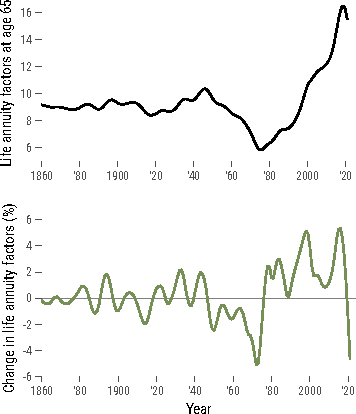
\includegraphics[width=0.5\linewidth]{Fig/lifeAnnuityFactorsAndChanges}
	\caption{{Life annuity factors, $\bar{a}_x(t)$, and relative change $\acute{\bar{a}}_x(t)$ calculated at age 65. Males, 1860-2021.}}
	\label{fig:Fig2}
\end{figure}


The upper panel of Figure \ref{fig:Fig2} presents life annuity factors, \( \bar{a}_x(t) \), from 1860 to 2021, calculated for males aged 65. During the second half of the 19th century and up until the 1940s, \( \bar{a}_{65}(t) \) remained relatively stable, exhibiting only small fluctuations. This period of stability was followed by a sharp decline that continued into the 1980s, after which an increasing trend persisted into recent years. 

The lower panel of Figure \ref{fig:Fig2} illustrates the changes in \( \bar{a}_{65}(t) \) through its relative derivative with respect to time \( t \) (i.e., \( \acute{\bar{a}}_{65}(t) \)). Positive values of \( \acute{\bar{a}}_{65}(t) \) indicate an upward trend in life annuity factors, whereas negative values signify a decline. In the following sections, we analyse the sources driving the time trend of \( \acute{\bar{a}}_{65}(t) \) using the equations developed in Section \ref{sec:TimeDynamics}.



\subsection{Contribution of Financial and Longevity Components to the Change in $\bar{a}_x(t)$}

As shown in Section \ref{sec:TimeDynamics}, when a single interest rate is used for each observation period, changes over time in \( \bar{a}_x(t) \) can be decomposed into longevity and financial components, expressed as 

\[
\acute{\bar{a}}_x(t) = \bar{\rho}(t) {H}^{p}_x(t) + \dot{\delta}(t) D^{c}_x(t).
\]

Each component is influenced by the time fluctuations of \( \mu(x,t) \) and \( \delta(s,t) \), represented by \( \bar{\rho}(t) \) and \( \dot{\delta}(t) \), respectively. These fluctuations are further modulated by the sensitivity of \( \bar{a}_x(t) \) to each factor, characterised by entropy (\( {H}^{p}_x(t) \)) and modified duration (\( {D}^{c}_x(t) \)). We begin by analysing the development of each component driving the time fluctuations in \( \bar{a}_x(t) \).

\begin{figure}[H]
	\centering
	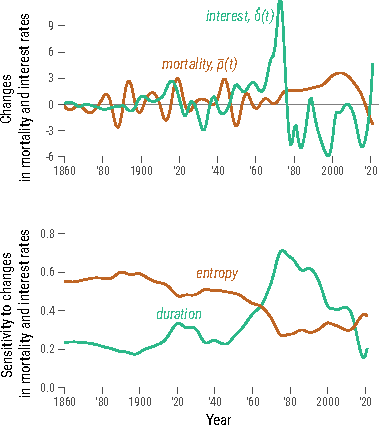
\includegraphics[width=0.5\linewidth]{Fig/changeMortalityInterestAndSensitivities}
	\caption{{Development in changes in mortality and interest and sensitivities. Upper panel shows the average mortality improvement ($\bar{\rho}(t)$), and change in interest rates ($\dot{\delta}(t)$). Lower panel depicts the entropy ($H$) and modified duration ($D$). Males at age 65, 1860-2021.}}
	\label{fig:Fig3}
\end{figure}


The upper panel of Figure \ref{fig:Fig3} shows that between 1860 and 1940, there were periods of both mortality improvement and deterioration (e.g., during the World Wars and the Spanish Flu pandemic). Starting in the 1980s, \( \bar{\rho}(t) \) increased steadily, reflecting average annual mortality improvements of 2\% to 3\%. In recent years, however, \( \bar{\rho}(t) \) has trended downward, reflecting the stagnation in mortality improvements in the United Kingdom, as documented by \citet{djeundje2022slowdown}. The substantial impact of the Covid-19 pandemic is evident in the sharp decline in \( \bar{\rho}(t) \) observed in 2020 and 2021.


With respect to interest rates, \( \dot{\delta}(t) \) remained relatively stable throughout most of the observation period, with some fluctuations between 1930 and 1950. Starting in the 1960s, \( \dot{\delta}(t) \) increased rapidly, peaking in the 1970s before declining sharply and turning negative, reflecting the prolonged decline in interest rates observed through the 2010s. However, since the Covid-19 pandemic, interest rates have risen rapidly once again.


The impact of fluctuations in \( \bar{\rho}(t) \) and \( \dot{\delta}(t) \) on the time dynamics of \( \bar{a}_x(t) \) is modulated by entropy (\( {H}^{p}_x(t) \)) and modified duration (\( {D}^{c}_x(t) \)). The lower panel of Figure \ref{fig:Fig3} indicates that, up until the 1960s, \( \bar{a}_x(t) \) was more sensitive to changes in mortality than to changes in interest rates, as entropy was higher than duration during this period. Starting in the 1960s, entropy exhibited a sharp decline, reaching its lowest point in the 1980s, before beginning to rise again.

Duration remained relatively constant from 1860 until the 1950s, when it began trending upward, peaking in the 1980s. Thereafter, duration declined through the 2010s, reflecting the low-interest rate environment during this period, which reduced sensitivity to interest rate changes. More recently, duration has increased in tandem with the rapid rise in interest rates.

As noted in Figure \ref{fig:Fig3}, there were specific years when duration and entropy were nearly identical. For example, in 1964, both duration and entropy were approximately 0.42, whereas in 2014, these values were around 0.32, indicating equal sensitivity of \( \bar{a}_x(t) \) to changes in mortality and interest rates during these years.

To further explore the interplay between entropy and duration, Table \ref{tab:entropyDuration} presents values for selected years. For instance, a proportional 1\% decline in mortality rates across all ages after 65 in 2021 would result in an increase of 0.37 in \( \bar{a}_{65}(t) \). Similarly, a constant 1\% decrease in interest rates during the same year would lead to an increase of 0.20 in \( \bar{a}_{65}(t) \).



\begin{table}[ht]
	\begin{tabular}{rccccc}
		\toprule
		& \multicolumn{5}{c}{\textbf{Year}}  \\

		& \textbf{1950} & \textbf{1980} & \textbf{2010 }& \textbf{2020} & \textbf{2021} \\
\hline
	\textit{Entropy} &  0.49    & 0.28     & 0.30     &   0.38 & 0.37  \\
	
		\textit{Duration} &  0.26    & 0.68     &  0.42    &     0.16 & 0.20\\
\bottomrule
	\end{tabular}
	 \caption{ Entropy and duration for male life annuities at age 65, selected years.}
	\label{tab:entropyDuration}   
\end{table}

These results stand in contrast to the findings of \citet{rabitti2020mortality}, who argued that duration is the primary driver of changes in life annuities. By contrast, Table \ref{tab:entropyDuration} underscores the interplay between mortality and interest rates, demonstrating that both factors contribute substantially to changes in life annuities during specific periods.

Using the equation \( \acute{\bar{a}}_x(t) = \bar{\rho}(t) {H}^{p}_x(t) + \dot{\delta}(t) D^{c}_x(t) \), the contributions of financial and longevity components to changes in life annuity factors are calculated. The upper panel of Figure \ref{fig:Fig4} presents \( \acute{\bar{a}}_{65}(t) \) (as shown in Figure \ref{fig:Fig2}), while the lower panel illustrates the respective contributions of financial and longevity components. Positive values indicate upward contributions, whereas negative values represent downward effects. Figure \ref{fig:Fig4} clearly highlights the significant roles that both longevity and financial risks play in shaping the long-term development of \( \bar{a}_x(t) \).


\begin{figure}[H]
	\centering
	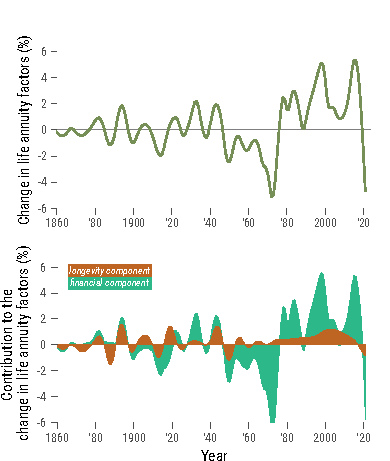
\includegraphics[width=0.5\linewidth]{Fig/decompositionLongTermSingleInterestRates}
	\caption{{Decomposition of changes over time in life annuity factors. Upper panel shows the relative change in a life annuity factor calculated at age 65 for males from 1860-2021. Lower panel shows the financial and longevity components that drive the relative change in the life annuity. }}
	\label{fig:Fig4}
\end{figure}

We identify five distinct periods during which annuity factors responded to specific changes in financial and longevity components. From 1860 to 1945, annuity factors remained stable, with modest contributions from both components. Between 1945 and 1970, annuity factors declined, driven primarily by the financial component. Around 1970, interest rates peaked, resulting in a pronounced negative contribution from the financial component. From 1970 to 2015, annuity factors increased due to positive contributions from both financial and longevity components. Since 2015, \( \bar{a}_x(t) \) has continued to rise, albeit with a diminished contribution from the longevity component, reflecting the deceleration in mortality improvements observed in the United Kingdom and other populations \citep{djeundje2022slowdown}. A new pattern has emerged since 2020, attributed to the Covid-19 pandemic, characterised by negative contributions from both the longevity and financial components.


\subsection{Age and Term Contributions}

Next, the longevity and financial components shown in Figure \ref{fig:Fig4} are further decomposed into contributions from age groups and yield curve terms. The yield curve for this analysis was constructed using government bonds (gilts) issued at various maturities \citep{BankOfEngland2024}. The analysis is restricted to the period from 1970 to 2021 due to data availability.

Figure \ref{fig:Fig5} illustrates the contributions of 10-year age groups (i.e., 65–74, 75–84, 85–94, 95–104) to the longevity component, as well as the corresponding contributions from yield curve terms (i.e., 0–9, 10–19, 20–29, 30–39 years). The figure reveals that the primary drivers of changes in \( \bar{a}_{65}(t) \) stem from the age group 65–74 and interest rates with terms below 10 years.

\begin{figure}[H]
	\centering
	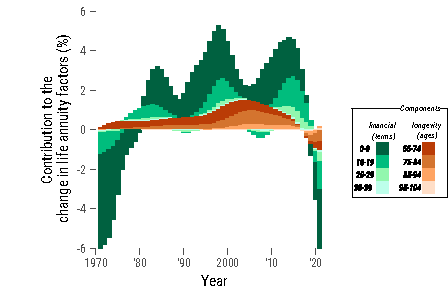
\includegraphics[width=0.6\linewidth]{Fig/ageTermStructureDescomposition}
	\caption{{Age and term attributions to changes over time in life annuity factors calculated at ages 65. Males, 1970-2021.}}
	\label{fig:Fig5}
\end{figure}

Figure \ref{fig:Fig6} provides a closer examination of age-term sensitivities for the years 1990, 2000, 2015, and 2021. The upper left panel shows that in 1990, the duration for yield terms of 0–9 years and the entropy for the age group 65–74 were significantly higher than for other age-term groups, indicating heightened sensitivity of annuities to changes in mortality and interest rates within these age-term ranges. 

\begin{figure}[H]
	\centering
	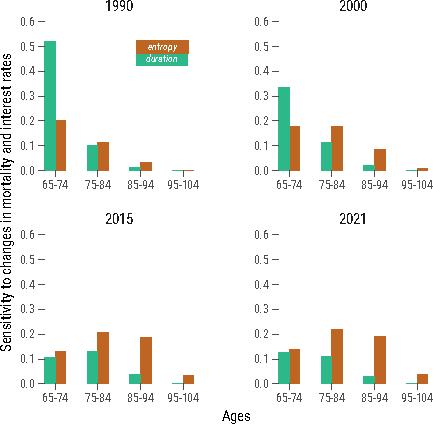
\includegraphics[width=0.6\linewidth]{Fig/attributionEntropyDuration}
	\caption{{Entropy and duration by age groups. Males, 1990, 2000, 2015 and 2021.}}
	\label{fig:Fig6}
\end{figure}


However, this sensitivity has shifted over time. By 2015, higher values for duration and entropy had transitioned to later age-term groups. For instance, by 2015, entropy had significantly exceeded duration, with increased sensitivity to mortality changes observed in the 75–94 age group. This pattern persisted into 2021, reflecting the economic-demographic conditions during the Covid-19 pandemic years.

\subsection{Cause of Death Contributions}

Finally, in this section, we examine the causes of death driving changes in observed life annuity factors using the equation 

\[
\acute{\bar{a}}_x(t) = \sum_{i=1}^{n} \bar{\rho}^i_x(t) {H}^i_x(t) + \bar{\upvarphi}(t) {D}^P_x(t),
\]

where the longevity component is represented by \( \sum_{i=1}^{n} \bar{\rho}^i_x(t) {H}^i_x(t) \), and \( n \) causes of death are considered in the analysis.

We use cause-specific mortality rates from the Human Cause-of-Death Data Series, retrieved from the \citet{HCD2024}, covering the period from 2001 to 2020. Causes of death in this database are categorised according to the ICD-10 International Classification of Diseases. For illustrative purposes, six major categories are analysed: neoplasms (ICD-10 codes C00–D48), heart diseases (ICD-10 codes I00–I52), cerebrovascular diseases (ICD-10 codes G45, I60–I69), respiratory diseases (ICD-10 codes J00–J22, J30–J98, U04, U07–U10), and other causes. Covid-19 (ICD-10 code U07) is included in the category of respiratory diseases exclusively for the year 2020, as it marked the first year the disease was observed.

\begin{figure}[H]
	\centering
	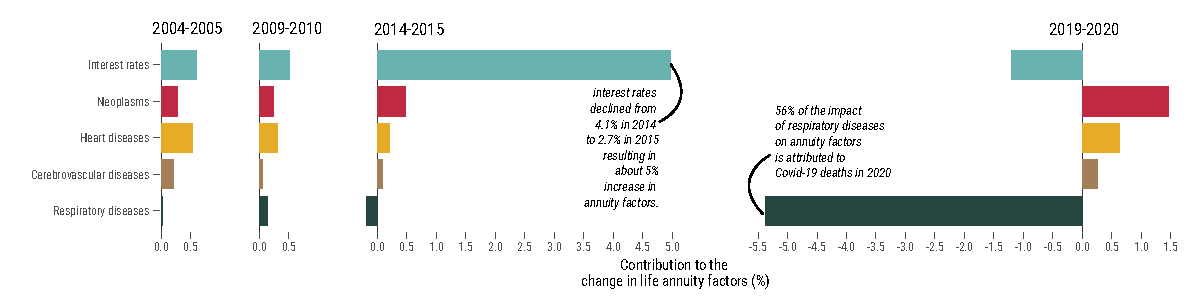
\includegraphics[width=1\linewidth]{Fig/attributionCauseOfDeathInLine}
	\caption{{Causes of death contributions to the change in life annuity factors. Males, 2004-2005, 2009-2010, 2014-2015 and 2019-2020.}}
	\label{fig:Fig7}
\end{figure}

Figure \ref{fig:Fig7} illustrates the cause-specific contributions to changes in life annuity factors for the periods 2004–2005, 2009–2010, 2014–2015, and 2019–2020. Positive values represent increases in life annuity factors, while negative values indicate reductions. Contributions from changes in interest rates are also shown.

From 2004 to 2005, heart diseases were the leading cause of death contributing to changes in life annuity factors, followed by neoplasms and cerebrovascular diseases, with minor positive contributions from respiratory diseases. This result indicates that reductions in mortality due to heart diseases were primarily responsible for the observed increases in life annuity factors during these years. Notably, the contribution of heart diseases from 2004 to 2005 was similar in magnitude to the contribution from changes in interest rates (about 0.6\%).

From 2014 to 2015, neoplasms emerged as the primary cause of death contributing to increases in life annuity factors, followed by heart diseases. However, these increases were small compared to the impact of changes in interest rates. Significant reductions in interest rates during this period resulted in increases of approximately 5\% in life annuity factor values, as observed in the interest rate component.

From 2019 to 2020, the contribution of causes of death shifted considerably due to the emergence of Covid-19. High mortality from respiratory diseases accounted for a 5.4\% decrease in life annuity factors, with Covid-19 deaths representing 56\% of all respiratory disease-related deaths. Thus, it can be estimated that Covid-19 mortality contributed to a 3\% decline in life annuity factors at age 65. Interestingly, during this period, there were positive contributions from neoplasms and heart diseases. This phenomenon is likely linked to the Covid-19 pandemic, as fewer deaths were attributed to these causes due to the predominance of Covid-19-related mortality.

Understanding the sources of changes in life annuities is crucial for several reasons. First, it allows actuaries and risk managers to link fluctuations in life annuities to specific health trends, facilitating more thorough risk assessments. Second, it provides valuable insights into how improvements or setbacks in public health impact life annuity portfolios. For instance, advances in cancer treatment and cardiovascular care have significantly improved mortality rates in high-income countries \citep{weber2023gains}, contributing to rising life expectancies. In contrast, the Covid-19 pandemic has had a profound effect on the life annuity sector, as the mortality shock led to lower longevity expectations. These findings highlight the importance of incorporating cause-of-death analysis into actuarial practice, particularly when managing longevity risk in life annuity portfolios.


\FloatBarrier
\section{Time Dynamics of Reserves}\label{sec:Reserves}

In this section, we extend the equations developed in Section \ref{sec:TimeDynamics} and illustrated in Section \ref{sec:UK_Illustration} to incorporate a stochastic representation of the payment process and the corresponding reserves for life annuities. This extension establishes a connection with the Thiele differential equations and may enable the application of our results in risk management and solvency assessments.

Let us recall that in Section \ref{preliminaries}, we defined time variable \(t\) as the moment when information about the \textit{economic-demographic environment} becomes available and time variable \(u\) denote the \textit{time of valuation of the policy}. 

Let us now define a probability space \( \{\Omega, \mathcal{F}, \mathbb{P}\} \), with \(\textbf{F} = \{\mathcal{F}_t\}\) representing a family of sub-\(\sigma\)-algebras that encodes the information available at time \( t \) regarding the economic-demographic environment. Let \( I_{s} = \mathds{1}_{\{S_x > s\}} \) and \( \mathbb{E}[I_{s} | \mathcal{F}_t] = {}_s p_x(t) \), we define the payment process as \( dB(s) = b(s) I_{s} \, ds \), where \( b(s) \) is the continuous rate of benefit payments over the development of the policy for the insured life \( (x) \).


Consider the policy value evaluated at time \( u \), with information generated at time \( t \), denoted as \({}_u\mathcal{V}_x(t)\), such that:

\[
{}_u\mathcal{V}_x(t) = \frac{1}{v(u, t)} \int_u^{\infty} v(y, t) \, dB(y),
\]

where \( v(u, t) \) represents the discount factor at valuation time \( u \) with information at time \( t \), and \( B(y) \) is the benefit function at payment time \( y \). Notably, both mortality and interest rates are stochastic processes evaluated at time \( t \), as they are not deterministically known at the time of policy issuance (i.e., at time zero). Given the requirement for the pension fund to maintain sufficient reserves to cover the financial value of \({}_u\mathcal{V}_x(t)\) at all times, the prospective reserve can then be expressed as:

\begin{equation}\label{eq:Reserve1}
	{}_uV_x(t) = \mathbb{E}[{}_u\mathcal{V}_x(t) \cdot v(u,t) \,|\, \mathcal{F}_t] = \mathbb{E} \left[ \int_u^\infty v(y,t) \, dB(y) \,|\, \mathcal{F}_t \right],
\end{equation}
which reduces to
\begin{equation}\label{eq:Reserve2}
	{}_uV_x(t) = \int_u^\infty v(y,t) \, {}_yp_x(t) \, b(y) \, dy.
\end{equation}

As in Section \ref{sec:TimeDynamics}, we differentiate Equation (\ref{eq:Reserve2}) with respect to time $t$:
\begin{equation}\label{eq:DifferentiateReserveT}
	{}_u\dot{V}_x(t) = \int_u^\infty \dot{v}(y,t) \, {}_yp_x(t) \, b(y) \, dy + \int_u^\infty v(y,t) \, {}_y\dot{p}_x(t) \, b(y) \, dy.
\end{equation}

Differentiating both sides of \eqref{eq:DifferentiateReserveT} yields:
\begin{equation}\label{eq:DifferentiateReserveT2}
	\begin{split}
		{}_u\dot{V}_x(t) &= \int_u^\infty \upvarphi(y,t) \, \delta(y,t) \, {}_yV_x(t) \, dy + \int_u^\infty \rho(x+y,t) \, \mu(x+y,t) \, {}_yV_x(t) \, dy \\ 
		&= \int_u^\infty \upvarphi(y,t) \, {}_yW^V_x(t) \, dy + \int_u^\infty \rho(x+y,t) \, {}_yM^V_x(t) \, dy,
	\end{split}
\end{equation}
where ${}_yM^V_x(t) = \mu(x+y,t) \, {}_yV_x(t)$ is the attribution to mortality of the policy holder due to reaching age $(x+y)$, and ${}_yW^V_x(t) = \delta(y,t) \, {}_yV_x(t)$ is the interest earned on the amount of the reserve. Quantities $\rho(x+y,t)$ and $\upvarphi(y,t)$ denote changes at time $t$ in the demographic-economic environment where the reserve is evaluated. 


Similar to the deterministic case of a single annuity factor developed in Section \ref{sec:TimeDynamics}, we aim to derive a closed expression for the relative change in the actuarial reserve, denoted by ${}_u\acute{V}_x(t)$. Dividing Equation (\ref{eq:DifferentiateReserveT2}) by ${}_uV_x(t)$ results in:
\begin{equation}\label{eq:AccuteDifferential}
	{}_u\acute{V}_x(t) = \underbrace{{}_u\bar{\rho}_x(t) \cdot {}_uH_x^V(t)}_\text{longevity component} + \underbrace{{}_u\bar{\upvarphi}(t) \cdot {}_uD_x^V(t)}_\text{financial component},
\end{equation}
where ${}_u\bar{\rho}_x(t) = \frac{\int_u^\infty \rho(x+y,t) \, {}_yM^V_x(t) \, dy}{\int_u^\infty {}_yM^V_x(t) \, dy}$ is the average change in mortality at all ages, and ${}_u\bar{\upvarphi}(t) = \frac{\int_u^\infty \upvarphi(y,t) \, {}_yW^V_x(t) \, dy}{\int_u^\infty {}_yW_x(t) \, dy}$ is the average term-structure change in interest rates over all terms. The sensitivities of the reserve to changes in mortality and interest rates are given by ${}_uH_x^V(t) = \dfrac{\int_{u}^{\infty} {}_yM^V_x(t) \, dy}{{}_uV_x(t)}$ and ${}_uD_x^V(t) = \dfrac{\int_{u}^{\infty} {}_yW^V_x(t) \, dy}{{}_uV_x(t)}$, respectively.

The differential equation (\ref{eq:AccuteDifferential}) decomposes the changes in the reserve over time, where the effect of mortality improvements is modulated by entropy, and changes in the term structure of interest rates are modulated by duration. Similar to the deterministic case of a single annuity factor, each term in Equation (\ref{eq:AccuteDifferential}) can be further decomposed into age-term attributions and cause-specific contributions, using the expressions provided in Table \ref{table:Table1}.



\subsection{Time Dynamics over $u$ and the Relationship with Thiele Differential Equation}\label{sec:ThieleEquations}


Quantities \( \mu \) and \( \delta \) are not deterministically known at the time of policy issuance. In reality, the actuarial valuation of the reserve \( {}_uV_x(t) \) incorporates assumptions (and models) that provide a reasonable depiction of the \textit{economic-demographic environment} in which the policies operate. On the one hand, the differential equations in (\ref{eq:DifferentiateReserveT2}) and (\ref{eq:AccuteDifferential}) capture the time dynamics of the reserve with respect to changes over time in the assumptions used for the actuarial valuation, which are indexed by the time variable \( t \).

On the other hand, changes in the reserve \( {}_u\mathcal{V}_x(t) \) over the time horizon during which the policy is in force (i.e., the \textit{policy term}) are described by the well-known \textit{Thiele's differential equation}. These changes are indexed by the time variable \( u \). Thiele's differential equation is a widely used tool for constructing reserves for life annuities capturing the development of the components over time. Equation (\ref{eq:DifferentiateReserveT2}) and Thiele's differential equation are closely related, as they both describe the dynamics of the reserve. This close relationship will be explored further in what follows.

The Thiele's differential equation for the reserve \( {}_uV_x(t) \) is obtained by differentiating Equation (\ref{eq:Reserve2}) with respect to \( u \):
\begin{equation}\label{eq:Thiele}
	\begin{split}
		\dfrac{\partial {}_uV_x(t)}{\partial u}&= \mu(x+u,t){}_uV_x(t) + \delta(u,t){}_uV_x(t) - b(u) \\
		&= {}_uM^V_x(t) + {}_uW^V_x(t) - b(u)
	\end{split}
\end{equation}

Then, ${}_uM^V_x(t)$ and ${}_uW^V_x(t)$ represent the quantities introduced in Equation (\ref{eq:DifferentiateReserveT2}): ${}_uM^V_x(t) = \mu(x+u,t){}_uV(t)$, which represents the mortality attribution of the policyholder due to reaching age \( (x+u) \), and ${}_uW^V_x(t) = \delta(u,t){}_uV(t)$, which reflects the interest earned on the reserve amount ${}_uV(t)$. The quantity \( b(u) \) denotes the rate of benefit payments, corresponding to the process \( dB(u) = b(u) I_{u} \, du \).

The attributions ${}_uM^V_x(t)$ and ${}_uW^V_x(t)$ are evaluated using the economic-demographic information available at time \( t \). In the expression for ${}_u\dot{V}_x(t)$, shown in Equation (\ref{eq:DifferentiateReserveT2}), the attributions ${}_uM^V_x(t)$ and ${}_uW^V_x(t)$ are integrated over the remaining policy term \( [u, \infty) \). This indicates that quantity ${}_u\dot{V}_x(t)$ accounts for the total attributions of mortality and interest rates over the remaining policy term, modulated by changes in the economic-demographic information at time \( t \) (i.e., assumptions about interest rates and mortality). In other words, ${}_u\dot{V}_x(t)$ quantifies the effect of time-\( t \) developments in the actuarial assumptions on the reserve evaluated at time \( u \).

 
The relationship between ${}_u\dot{V}_x(t)$ and the Thiele's differential equation becomes clearer when differentiating ${}_u\dot{V}_x(t)$ with respect to $u$: 

\begin{equation}\label{eq:DifferentiateVdotWithRespectS}
\dfrac{\partial	{}_u\dot{V}_x(t)}{\partial u}= \rho(x+u,t) {}_uM^V_x(t)+ \upvarphi(u,t) {}_uW^V_x(t)
\end{equation}

Equation (\ref{eq:DifferentiateVdotWithRespectS}) captures the change in the reserve over two time dimensions: changes in the economic-demographic assumptions over time \( t \), and the development of the reserve over time \( u \). Here, the attributions \( {}_uM^V_x(t) \) and \( {}_uW^V_x(t) \) are modulated by the changes in mortality and interest rates via \( \rho(x+u,t) \) and \( \upvarphi(u,t) \).

Equation (\ref{eq:DifferentiateVdotWithRespectS}) extends the traditional Thiele’s differential equation by separating the sources of variation in the economic-demographic environment. Together with Equation (\ref{eq:DifferentiateReserveT2}), this equation has significant actuarial applications, such as in product development and risk management. Some of these applications, along with further developments, are discussed in the following section.

It is important to note that the rate of payment \( b(u) \) no longer appears in Equation (\ref{eq:DifferentiateVdotWithRespectS}). This is because the benefit payments evolve solely over the development of the contract, i.e., over the period \( [u, \infty) \), and do not depend on changes in the assumptions regarding the economic-demographic environment, i.e., changes at time \( t \). This assumption is reasonable, as benefit payments are typically adjusted over the length of the contract. However, this assumption can be modified to allow for the possibility of using \( b(u,t) \) instead.

Furthermore, it is possible that time \( t \) and \( u \) coincide, meaning that information about the economic-demographic environment is incorporated into the valuations at the same time the policy develops. However, in most cases, this is not necessarily true. In practice, a life insurance company or pension fund may perform continuous evaluations of the actuarial provision using market-based yield curves, where financial information is continuously updated. In such cases, \( t = u \) holds for interest rates. On the other hand, demographic statistics are typically published with some delay, and estimates of the force of mortality \( \mu \) are made over broader time intervals. As a result, the experience of contract development at time \( u \) often does not align with the pace at which demographic assumptions are updated at time \( t \). Additionally, there may be value in distinguishing between times \( t \) and \( u \) in Scandinavian-style life insurance products, where it is common to differentiate between deterministic \textit{first-order} actuarial bases, prudently set by the actuary, and \textit{second-order} actuarial bases, which are typically based on market models.


\subsection{Risk management applications}

The differential equations developed in Section \ref{sec:Reserves} facilitate the analysis of risk drivers in the development of reserves, aligning with contemporary risk management practices.

For example, the current version of Solvency II regulations stipulates that a company must hold capital requirements for longevity risk corresponding to a shock that results in an immediate 20\% reduction in mortality rates across all ages. This shock can be represented by the factor \( \bar{\rho} = 0.2 \), which can then be used to determine the percentage impact on the reserve through the equation 

\[
{}_u\acute{V}_x(t) = {}_u\bar{\rho}_x(t) \, {}_uH_x^V(t) + {}_u\bar{\upvarphi}(t) \, {}_uD_x^V(t).
\]

Further scenario-based shocks to mortality and interest rates can be applied to \( {}_u\acute{V}_x(t) \), where \( {}_u\bar{\rho}_x(t) \) and \( \bar{\upvarphi} \) are stressed. By using the duration and entropy, actuaries and risk managers can leverage this tool to assess the impact of insurance and financial risks on their life annuity portfolios.

Similarly, \( {}_u\bar{\rho}_x(t) \) and \( {}_u\bar{\upvarphi}(t) \) can be modeled as stochastic processes adapted to a filtration \( \textbf{G} = \{\mathcal{G}_t\}_{t \ge 0} \) such that 

\[
{}_u{\rho}^{\bf{G}}_x(t) = \mathbb{E}[{}_u\bar{\rho}_x(t) \mid \mathcal{G}_t] \quad \text{and} \quad {}_u{\upvarphi}^{\bf{G}}(t) = \mathbb{E}[{}_u\bar{\upvarphi}(t) \mid \mathcal{G}_t].
\]

In this framework, the source of randomness in these stochastic processes can be explicitly modeled using forecasting models, enabling stochastic simulations. The resulting simulations of changes in reserves can then be used to calculate common risk metrics, such as Value at Risk, Expected Shortfall, and others. The ability to perform stochastic simulations of \( {}_u{\rho}^{\bf{G}}_x(t) \) and \( {}_u{\upvarphi}^{\bf{G}}(t) \) is particularly valuable in Asset-Liability modelling, where the impact of stochastic shocks on reserves is translated into corresponding management actions aimed at mitigating the associated risks.

The risk analysis can be further extended by examining the age-specific and term-specific stochastic variations in \( {}_u{\rho}^{\bf{G}}_x(t) \) and \( {}_u{\upvarphi}^{\bf{G}}(t) \), adapting the formulas presented in Table \ref{table:Table1}. These equations enable further segregation by sub-population, risk factors, or any cause of death.



\section{Concluding Remarks}\label{sec:6_Conclusion}

In this article, we introduced a set of differential equations to uncover the underlying sources of change in life annuities and their associated reserves. These equations are concise, intuitive, and readily implementable with real-world data, representing a significant expansion of the mathematical toolkit available for pension and life insurance analysis.

The primary advantage of our approach lies in its ability to capture the simultaneous variation of mortality and interest rates. Our key equation demonstrates that changes in life annuities over time are driven not only by fluctuations in mortality and interest rates but also by their sensitivities to these factors, encapsulated through entropies and durations.

Traditionally, actuaries and risk managers have analysed changes in interest and mortality rates in isolation, often overlooking their simultaneous interaction. However, in reality, mortality and interest rates evolve together, with durations and entropies dynamically adjusting to the changing economic-demographic environment. Although the correlation between mortality and interest rates remains an open question, both clearly influence the value of life annuities and reserves. The differential equations presented here explicitly account for this simultaneous behaviour and the evolving sensitivities to mortality and interest rates.

A notable strength of these equations is their flexibility. Being model-free, they provide general expressions for the time dynamics of life annuities, avoiding restrictive assumptions about the underlying demographic or economic environment. One of their most valuable applications lies in monitoring the sources of change in life annuity portfolios using real-world data. To illustrate this, we applied our framework to over two centuries of data from the United Kingdom, yielding data-driven insights into the evolution of life annuity portfolios at granular levels, such as age-term-specific contributions and causes of death.


While this article focuses primarily on the time dynamics of life annuities and reserves, the framework we propose is readily extendable to other life-contingent products. Future developments could incorporate lump sums, expenses, and more complex payment processes, broadening the applicability of this approach.

An important direction for future research is the adaptation of these equations to a multi-state Markov framework, enabling the modelling of risks beyond mortality (e.g. disability). Such an extension would allow for the development of state-specific sensitivities, explicitly accounting for variations in age-term intensities across different states.

%Looking ahead, we anticipate that the differential equations developed in this paper could find broad applications in both actuarial practice and academic research. Regardless of the specific application, the ability of these equations to provide valuable insights into the time dynamics of life annuities ensures their continued relevance and utility in advancing the field.

Looking ahead, we hope that the differential equations developed in this paper may find applications in both actuarial practice and academic research. While their full potential remains to be explored, we believe they offer the ability to provide valuable insights into the time dynamics of life annuities, particularly in understanding the interplay between longevity and financial risk. In doing so, they may contribute to a deeper understanding of economic-demographic interactions in long-term financial products, with implications for product design, solvency assessment, and risk management.

\newpage

\bibliographystyle{apalike}
%\bibliography{/Users/Jesus/Documents/Papers/BibTex/Proposal}
%\bibliography{C:/Users/jmartinez/OneDrive - Syddansk Universitet/Papers/BibTeX/Proposal.bib}

\bibliography{library}

\newpage


\FloatBarrier
\newpage
\appendix
\section{Appendix}


\subsection{Entropy with Constant Changes in $\mu(x+s,t)$}\label{sec:EntropyConst}

To measure constant changes we make $\mu(s,t)+\gamma$, then

\begin{equation}\label{eq:EntropyConst1}
\begin{split}
\bar{a}_{x}(t) &= \int_0^\infty{v}(s,t) e^{-\int_{0}^{s} [\mu(x+y,t)+\gamma]dy}ds \\
&= \int_0^\infty {v}(s,t)e^{-\int_{0}^{s} \mu(x+y,t)dy} e^{-\gamma s}ds \\
&= \int_0^\infty {v}(s,t){}_sp_x(t) e^{-\gamma s}ds \\
\end{split}
\end{equation}

We expand $e^{-\gamma s}$ to $1-\gamma s+\frac{\gamma^2}{2} s^{2} +...$, so that


\begin{equation}\label{eq:EntropyConst2}
\begin{split}
\bar{a}_{x}(t) &= \int_0^\infty {}_sp_x(t) {v}(s,t)[1-\gamma s+\frac{\gamma^2}{2} s^{2} +...]ds
\end{split}
\end{equation}

We take the derivative $\bar{a}_{x}(t)$ with respect to $\gamma$ and evaluate $\gamma=0$


\begin{equation}\label{eq:EntropyConst3}
\begin{split}
{H}^{c}_x(t)&=\frac{1}{\bar{a}_x(t)}\frac{\partial \bar{a}_x(t)}{\partial \gamma} \bigg\rvert_{\gamma=0}\\
&= -\frac{\int_0^\infty s {}_sp_x(t) {v}(s,t)ds}{\bar{a}_x(t)} \\
&= \frac{{h}^{c}_x(t)}{\bar{a}_x(t)},
\end{split}
\end{equation}

where ${h}^{c}_x(t)=-\int_0^\infty s {}_sp_x(t) {v}(s,t)ds$



\subsection{Alternative Expression for ${H}^{p}_{x}(t)$}\label{sec:EntropyAlt}

\begin{equation} \label{eq:EntropyAnnuityA1}
\begin{split}
{H}^{p}_{x}(t) &= -\frac{ \int_{0}^{\infty}{}_sp_x(t)\ln[{}_sp_x(t)] e^{-\int_{0}^{s}\delta(y,t)dy} ds}{\int_0^\infty {}_sp_x(t) e^{-\int_{0}^{s}\delta(y,t)dy} ds}\\
&= \frac{\int_0^\infty {}_sp_x(t) {v}(s,t) \int_0^s \mu(x+y,t) dy\,ds}{\bar{a}_x(t)}\\
&= \frac{\int_0^\infty  \mu(x+s,t) \int_s^\infty {}_yp_x(t) {v}(y,t)  dy\,ds}{\bar{a}_x(t)}\\
&= \frac{\int_0^\infty  \mu(x+s,t)  {}_sp_x(t) {v}(s,t) \int_s^\infty \frac{ {}_yp_x(t) {v}(y,t)}{ {}_sp_x(t) {v}(s,t)}  dy\,ds}{\bar{a}_x(t)}\\
&=  \frac{\int_0^\infty \mu(x+s,t)   {}_sp_x(t) {v}(s,t) \bar{a}_{x+s}(t) ds}{\bar{a}_x(t)} \\
&=  \frac{\int_0^\infty \mu(x+s,t)  {}_s|\bar{a}_x(t) ds}{\bar{a}_x(t)} \\
&=  \frac{{h}^{p}_{x}(t)}{\bar{a}_x(t)}, \\
\end{split}
\end{equation}

where ${h}^{p}_{x}(t)=\int_0^\infty \mu(x+s,t)   {}_s|\bar{a}_x(t) ds$.



\subsection{Duration with Constant Changes in $\delta(s,t)$}\label{sec:DurConst}

To measure constant changes we make $\delta(s,t)+\gamma$, then

\begin{equation}\label{eq:DurationConst11}
\begin{split}
\bar{a}_{x}(t) &= \int_0^\infty {}_sp_x(t) e^{- \int_{0}^{s} [\delta(y,t)+\gamma]dy}ds \\
&= \int_0^\infty {}_sp_x(t) e^{- \int_{0}^{s}\delta(y,t)dy}e^{-\gamma s}ds \\
&= \int_0^\infty {}_sp_x(t) {v}(s,t)e^{-\gamma s}ds
\end{split}
\end{equation}

We expand $e^{-\gamma s}$ to $1-\gamma s+\frac{\gamma^2}{2} s^{2} +...$, so that


\begin{equation}\label{eq:DurationConst1}
\begin{split}
\bar{a}_{x}(t) &= \int_0^\infty {}_sp_x(t) {v}(s,t)[1-\gamma s+\frac{\gamma^2}{2} s^{2} +...]ds
\end{split}
\end{equation}

We take the derivative $\bar{a}_{x}(t)$ with respect to $\gamma$ and evaluate $\gamma=0$


\begin{equation}\label{eq:DurationConst2}
\begin{split}
{D}^{c}_x(t)&=-\frac{1}{\bar{a}_x(t)}\frac{\partial \bar{a}_x(t)}{\partial \gamma} \bigg\rvert_{\gamma=0}\\
              &= \frac{\int_0^\infty s {}_sp_x(t) {v}(s,t)ds}{\bar{a}_x(t)} \\
              &= \frac{{d}^{c}_x(t)}{\bar{a}_x(t)},
\end{split}
\end{equation}

where ${d}^{c}_x(t)=\int_0^\infty s {}_sp_x(t) {v}(s,t)ds$



\subsection{Duration with Proportional Changes in $\delta(s,t)$} \label{sec:DurProp}

To calculate duration with proportional changes in $\delta(s,t)$, we assume that $\gamma$ is a small number such that $\delta(s,t)(1+\gamma)$ and  ${v}(s,t)=e^{-\int_0^{s}  \delta(y,t)(1+\gamma)dy}$.


\begin{equation}\label{eq:DurationProp1}
\begin{split}
\bar{a} _x(t) &= \int_0^\infty {}_sp_x(t) e^{-\int_0^{s}\delta(y,t)(1+\gamma)dy}ds \\
&= \int_0^\infty {}_sp_x(t) e^{-\int_0^{s}\delta(y,t)dy}e^{-\int_0^{s}\delta(y,t)\gamma dy}ds \\
&= \int_0^\infty {}_sp_x(t) v(s,t)v(s,t)^{\gamma}ds \\
\end{split}
\end{equation}


We expand $v(s,t)^{\gamma}$ to $1+\ln(v(s,t)) \gamma+{\ln(v(s,t))}^2 \frac{\gamma^2}{2}+...$, so that


\begin{equation}\label{eq:DurationProp2}
\begin{split}
\bar{a}_x(t) &= \int_0^\infty {}_sp_x(t) v(s,t)[1+\ln(v(s,t)) \gamma+{\ln(v(s,t))}^2 \frac{\gamma^2}{2}+...]ds\\
\end{split}
\end{equation}


To calculate the duration ${D}^{p}_{x}(t)$ we take the derivative of the expression above with respect to $\gamma$ and make $\gamma=0$

\begin{equation}\label{eq:DurationProp3}
\begin{split}
{D}^{p}_{x}(t)&=-\frac{1}{\bar{a}_x(t)}\frac{\partial \bar{a}_x(t)}{\partial \gamma} \bigg\rvert_{\gamma=0} \\
&= -\frac{\int_0^\infty {}_sp_x(t) v(s,t) \ln(v(s,t))ds}{\bar{a}_x(t)} \\
\end{split}
\end{equation}


Equation \ref{eq:DurationProp3} can be re-expressed as 


\begin{equation}\label{eq:DurationProp4}
\begin{split}
{D}^{p}_{x}(t) &= -\frac{\int_0^\infty {}_sp_x(t) v(s,t) \ln(v(s,t))ds}{\bar{a}_x(t)}\\
&= \frac{\int_0^\infty {}_sp_x(t) v(s,t) \int_0^{s} \delta(y,t)dy ds }{\bar{a}_x(t)}\\
&= \frac{\int_0^\infty \delta(s,t)  \int_{s}^{\infty} {}_{y}p_x(t) v(y,t)dy ds }{\bar{a}_x(t)}\\
&= \frac{\int_0^\infty \delta(s,t) {}_sp_x(t) v(s,t) \bar{a}_{x+s}(t)  ds }{\bar{a}_x(t)}\\
&= \frac{\int_0^\infty \delta(s,t) {}_s|\bar{a}_x(t) ds}{\bar{a}_x(t)} \\
&= \frac{{d}^{p}_{x}(t)}{\bar{a}_x(t)}.
\end{split}
\end{equation}



where ${d}^{p}_{x}(t)=\int_0^\infty \delta(s,t) {}_s|\bar{a}_x(t) ds$.

\counterwithin{figure}{section}
\setcounter{figure}{0}
\subsection{Figures}
\begin{figure}[!ht]
	\centering
	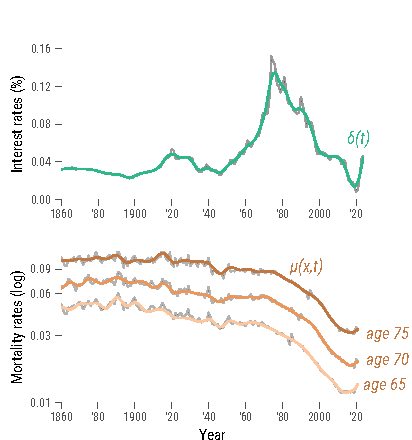
\includegraphics[width=0.6\linewidth]{Fig/interestMortalityRates}
	\caption{{Interest and mortality rates for the United Kingdom. Males, 1860-2021.}}
	\label{fig:Fig1}
\end{figure}

\end{document}
